\documentclass[a4paper, 12pt, english]{article}

% \usepackage[portuges]{babel}
\usepackage[utf8]{inputenc}
\usepackage{amsmath,amssymb}
\usepackage{graphicx}
\usepackage{subfig}
\usepackage[colorinlistoftodos]{todonotes}

\usepackage{indentfirst}
\usepackage{verbatim}
\usepackage{textcomp}
\usepackage{gensymb}
\usepackage{float}
\usepackage{pgfplots}
\pgfplotsset{
	scale only axis,
	xmin=0, xmax=0.06,
	y axis style/.style={
			yticklabel style=#1,
			ylabel style=#1,
			y axis line style=#1,
			ytick style=#1
		}
}

\usepackage{relsize}

\usepackage{lipsum}% http://ctan.org/pkg/lipsum
\usepackage{xcolor}% http://ctan.org/pkg/xcolor
\usepackage{xparse}% http://ctan.org/pkg/xparse
\NewDocumentCommand{\myrule}{O{1pt} O{2pt} O{black}}{%
	\par\nobreak % don't break a page here
	\kern\the\prevdepth % don't take into account the depth of the preceding line
	\kern#2 % space before the rule
	{\color{#3}\hrule height #1 width\hsize} % the rule
	\kern#2 % space after the rule
	\nointerlineskip % no additional space after the rule
}
\usepackage[section]{placeins}

\usepackage{booktabs}
\usepackage{colortbl}%
\newcommand{\myrowcolour}{\rowcolor[gray]{0.925}}

\usepackage[obeyspaces]{url}
\usepackage{etoolbox}
\usepackage[colorlinks,citecolor=black,urlcolor=blue,bookmarks=false,hypertexnames=true]{hyperref}

\usepackage{geometry}
\geometry{
	paper=a4paper, % Change to letterpaper for US letter
	inner=3cm, % Inner margin
	outer=3cm, % Outer margin
	bindingoffset=.5cm, % Binding offset
	top=2cm, % Top margin
	bottom=2cm, % Bottom margin
	%showframe, % Uncomment to show how the type block is set on the page
}
\usepackage{fancyhdr}

% Define header and footer
\pagestyle{fancy}
\fancyhf{}
\lhead{ENER 104L}
\rhead{iSciM, Habib University} % Right-aligned page number in the header
\rfoot{\thepage} % Right footer text
%*******************************************************************************%
%************************************START**************************************%
%*******************************************************************************%
\begin{document}

%************************************TITLE PAGE**************************************%
\begin{titlepage}
	\begin{center}
		\textbf{\LARGE Habib University}\\[0.5cm]
		\textbf{\large iSciM}\\[0.2cm]
		\textbf {\large Fall 2023}\\[0.2cm]
		\vspace{20pt}
		
\includegraphics[width=5cm]{../habiblogo.jpg}\\[1cm]
		\par
		\vspace{20pt}
		\textbf{\Large ENER 104L RENEWABLE ENERGY}\\
		\vspace{15pt}
		\myrule[1pt][7pt]
		\textbf{\LARGE  LABORATORY REPORT 10}\\
		\vspace{15pt}
		\textbf{\large Ambient Heat}\\
		\myrule[1pt][7pt]
		\vspace{25pt}
		\begin{tabular}{@{}p{5cm}p{3cm}@{}}
			\textbf{\large Student Name} & \textbf{\large Student ID} \\
			Ali Asghar Yousuf            & ay06993                    \\ % No1 
			Syed Ibrahim Ali Haider      & sh06565                    \\ % No2
		\end{tabular}

		\vspace{10pt}
		\begin{tabular}{@{}p{5cm}p{3cm}@{}}
			\textbf{\large Group Name} & \textbf{\large Group No.} \\
			Insane Fr                  & 1                         \\
		\end{tabular}

		\vspace{45pt}
		\textbf {\large Lab Instructors:}\\[0.2cm]
		\Large {Paishwa Naqvi}\\[0.1cm]
		\Large {Mah Noor Jamil}\\[0.1cm]
		\Large {Amber Talat}\\[0.1cm]
	\end{center}

	\par
	\vfill
	\begin{center}
		\textbf{\today}\\
	\end{center}

\end{titlepage}

%************************************TABLE OF CONTENTS**************************************%

%  %Sumário
%  \newpage
%  \tableofcontents
%  \thispagestyle{empty}
%  %End Sumário

%********************************%
%***********SECTION 1************%
%********************************%
\newpage
\section{Objectives}
\begin{itemize}
	\item To understand the concept of ambient heat.
	\item To understand the working of a thermogenerator.
	\item Observe the effect of temperature on the output voltage of a thermogenerator.
	\item Observe the difference in the working of the thermogenerator when the hot and
	      cold sides are interchanged.
\end{itemize}

\section{Abstract}

\section{Result and Analysis}
\subsection{Part A}
\subsubsection{Experiment 1}

\begin{table}[H]
	\centering
	\caption{Part A Experiment 1}
	\label{tab:partA1}
	\begin{tabular}{@{}lll@{}}
		\toprule
		\textbf{Side} & \textbf{Type} & \textbf{Voltage (V)} \\ \midrule
		Upper         & Warm          & 0.06                 \\
		Upper         & Cold          & -0.115               \\
		Under         & Warm          & -0.07                \\
		Under         & Cold          & 0.072                \\ \bottomrule
	\end{tabular}
\end{table}

\subsubsection{Experiment 2}
\begin{table}[H]
	\centering
	\caption{Part A Experiment 2}
	\label{tab:partA2}
	\begin{tabular}{@{}llll@{}}
		\toprule
		\textbf{Time (s)} & \textbf{Voltage (V)} & \textbf{Observation}   \\ \midrule
		0                 & -0.120                    & No movement of the fan \\
		15                & -0.138               & No movement of the fan \\
		30                & -0.14                & No movement of the fan \\
		45                & -0.152               & No movement of the fan \\
		60                & -0.135               & No movement of the fan \\
		75                & -0.23                & No movement of the fan \\
		90                & -0.116               & No movement of the fan \\
		105               & -0.111               & No movement of the fan \\
		120               & -0.105               & No movement of the fan \\
		135               & -0.1                 & No movement of the fan \\
		150               & -0.096               & No movement of the fan \\
		165               & -0.09                & No movement of the fan \\
		180               & -0.088               & No movement of the fan \\ \bottomrule
	\end{tabular}
\end{table}

\begin{figure}[H]
	\centering
	\begin{tikzpicture}
		\begin{axis}[
				width=0.8\textwidth,
				xlabel={Time (s)},
				ylabel={Voltage (V)},
				ylabel style={at={(axis description cs:-0.05,0.45)}, anchor=west},
				xmin=0, xmax=180,
				ymin=-0.2, ymax=0,
				y dir=reverse,
			]
			\addplot[
				mark=x, mark options={color=blue}, draw=blue,
			] table [x=T, y=V] {
					T  V
					0           -0.120
					15          -0.138
					30          -0.14
					45          -0.152
					60          -0.135
					75          -0.123
					90          -0.116
					105         -0.111
					120         -0.105
					135         -0.1
					150         -0.096
					165         -0.09
					180         -0.088
				};
		\end{axis}
	\end{tikzpicture}
	\caption{Voltage vs Time}
	\label{fig:a2}
\end{figure}

\subsubsection{Experiment 3}

\begin{table}[H]
	\centering
	\caption{Part A Experiment 3}
	\label{tab:partA3}
	\begin{tabular}{@{}llll@{}}
		\toprule
		\textbf{Time (s)} & \textbf{Voltage (V)} & \textbf{Observation}   \\ \midrule
		0                 & -0.120                    & No movement of the fan \\
		15                & -0.125               & No movement of the fan \\
		30                & -0.146               & No movement of the fan \\
		45                & -0.151               & No movement of the fan \\
		60                & -0.15                & No movement of the fan \\
		75                & -0.146               & No movement of the fan \\
		90                & -0.14                & No movement of the fan \\
		105               & -0.134               & No movement of the fan \\
		120               & -0.129               & No movement of the fan \\
		135               & -0.125               & No movement of the fan \\
		150               & -0.121               & No movement of the fan \\
		165               & -0.117               & No movement of the fan \\
		180               & -0.114               & No movement of the fan \\ \bottomrule
	\end{tabular}
\end{table}

\begin{figure}
	\centering
	\begin{tikzpicture}
		\begin{axis}[
				width=0.8\textwidth,
				xlabel={Time (s)},
				ylabel={Voltage (V)},
				ylabel style={at={(axis description cs:-0.05,0.45)}, anchor=west},
				xmin=0, xmax=180,
				ymin=-0.2, ymax=0,
				y dir=reverse,
			]
			\addplot[
				mark=x, mark options={color=blue}, draw=blue,
			] table [x=T, y=V] {
					T  V
					0           -0.120
					15          -0.125
					30          -0.146
					45          -0.151
					60          -0.15
					75          -0.146
					90          -0.14
					105         -0.134
					120         -0.129
					135         -0.125
					150         -0.121
					165         -0.117
					180         -0.114
				};
		\end{axis}
	\end{tikzpicture}
	\caption{Voltage vs Time}
	\label{fig:a3}
\end{figure}

\subsection{Part B}

\begin{table}[H]
	\centering
	\caption{Part B Experiment 1}
	\label{tab:partB1}
	\begin{tabular}{@{}llll@{}}
		\toprule
		\textbf{Time (min)} & \textbf{Voltage (V)} & \textbf{Water Temp. (\degree C)} & \textbf{Block Temp. (\degree C)} \\ \midrule
		0                   & 0.000                & 50                               & 24                               \\
		1                   & 0.240                & 49                               & 25                               \\
		2                   & 0.192                & 46                               & 26                               \\
		3                   & 0.173                & 43                               & 27                               \\
		4                   & 0.153                & 42                               & 28                               \\
		5                   & 0.142                & 40                               & 28                               \\
		6                   & 0.132                & 40                               & 28                               \\
		7                   & 0.124                & 38                               & 28                               \\
		8                   & 0.111                & 37                               & 28                               \\
		9                   & 0.100                & 47                               & 28                               \\
		10                  & 0.094                & 36                               & 28                               \\
		11                  & 0.086                & 35                               & 28                               \\
		12                  & 0.081                & 34                               & 28                               \\
		13                  & 0.076                & 34                               & 28                               \\
		14                  & 0.071                & 33                               & 28                               \\
		15                  & 0.071                & 33                               & 28                               \\ \bottomrule
	\end{tabular}
\end{table}

\begin{figure}[H]
	\centering
	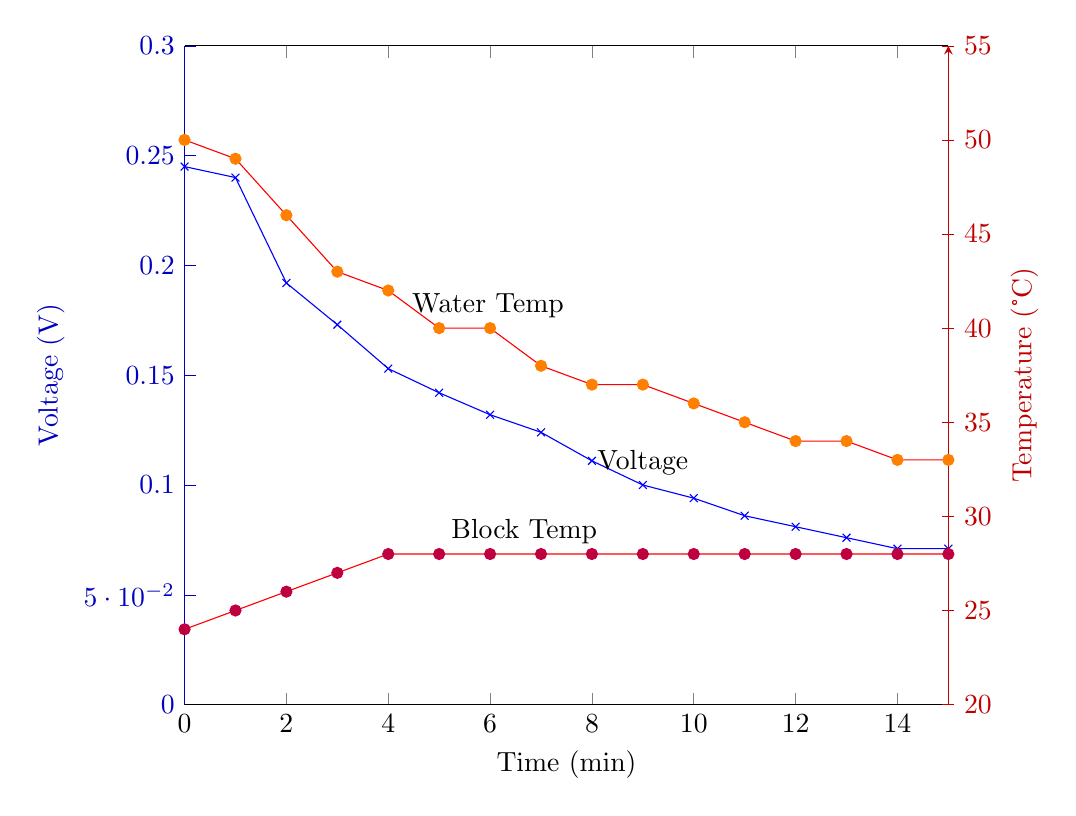
\begin{tikzpicture}
		\begin{axis}[
				width=0.8\textwidth,
				xlabel={Time (min)},
				ylabel={Voltage (V)},
				axis y line*=left,
				xmin=0, xmax=15,
				ymin=0, ymax=0.3,
				y axis style=blue!75!black,
			]
			\addplot[
				mark=x, mark options={color=blue}, draw=blue,
			] table [x=T, y=V] {
					T  V
					0           0.245
					1           0.240
					2           0.192
					3           0.173
					4           0.153
					5           0.142
					6           0.132
					7           0.124
					8           0.111
					9           0.100
					10          0.094
					11          0.086
					12          0.081
					13          0.076
					14          0.071
					15          0.071
				} node [pos=0.6, above] {Voltage};
		\end{axis}
		\begin{axis}[
				width=0.8\textwidth,
				axis y line=right,
				ylabel={Temperature (\degree C)},
				axis x line=none,
				xmin=0, xmax=15,
				ymin=20, ymax=55,
				y axis style=red!75!black,
			]
			\addplot[
				mark=*, mark options={color=orange}, draw=red
			] table [x=T, y=Wt] {
					T  Wt
					0           50
					1           49
					2           46
					3           43
					4           42
					5           40
					6           40
					7           38
					8           37
					9           37
					10          36
					11          35
					12          34
					13          34
					14          33
					15          33
				} node [pos=0.5, above] {Water Temp};

			\addplot[
				mark=*, mark options={color=purple}, draw=red
			] table [x=T, y=Bt] {
					T  Bt
					0           24
					1           25
					2           26
					3           27
					4           28
					5           28
					6           28
					7           28
					8           28
					9           28
					10          28
					11          28
					12          28
					13          28
					14          28
					15          28
				} node [pos=0.5, above] {Block Temp};
		\end{axis}
	\end{tikzpicture}
	\caption{Voltage and Temperature vs Time}
	\label{fig:graph}
\end{figure}

\section{Conclusion}

\end{document}